% Attack Scenarios Comparison Diagram
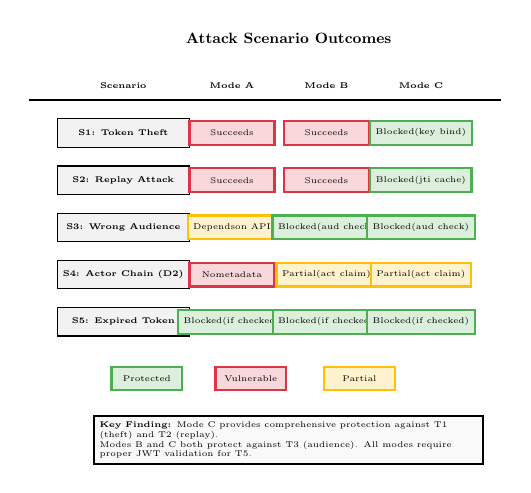
\begin{tikzpicture}[scale=0.6, every node/.style={scale=0.6}, font=\tiny]

\definecolor{failgreen}{RGB}{76,175,80}
\definecolor{successred}{RGB}{220,53,69}
\definecolor{partialyellow}{RGB}{255,193,7}

\tikzset{
    scenario/.style={rectangle, minimum width=2.8cm, minimum height=0.6cm,
                     text centered, draw=black, fill=gray!10, font=\tiny\bfseries},
    pass/.style={rectangle, minimum width=1.8cm, minimum height=0.5cm,
                 text centered, draw=failgreen, thick, fill=failgreen!20, font=\tiny},
    fail/.style={rectangle, minimum width=1.8cm, minimum height=0.5cm,
                 text centered, draw=successred, thick, fill=successred!20, font=\tiny},
    partial/.style={rectangle, minimum width=1.8cm, minimum height=0.5cm,
                    text centered, draw=partialyellow, thick, fill=partialyellow!20, font=\tiny},
}

% Title
\node[font=\small\bfseries] at (0,6) {Attack Scenario Outcomes};

% Column headers
\node[font=\tiny\bfseries] at (-3.5,5) {Scenario};
\node[font=\tiny\bfseries] at (-1.2,5) {Mode A};
\node[font=\tiny\bfseries] at (0.8,5) {Mode B};
\node[font=\tiny\bfseries] at (2.8,5) {Mode C};

% Horizontal line
\draw[thick] (-5.5,4.7) -- (4.5,4.7);

% S1: Token Theft
\node[scenario] (s1_label) at (-3.5,4) {S1: Token Theft};
\node[fail] (s1_a) at (-1.2,4) {Succeeds};
\node[fail] (s1_b) at (0.8,4) {Succeeds};
\node[pass] (s1_c) at (2.8,4) {Blocked\\(key bind)};

% S2: Replay Attack
\node[scenario] (s2_label) at (-3.5,3) {S2: Replay Attack};
\node[fail] (s2_a) at (-1.2,3) {Succeeds};
\node[fail] (s2_b) at (0.8,3) {Succeeds};
\node[pass] (s2_c) at (2.8,3) {Blocked\\(jti cache)};

% S3: Wrong Audience
\node[scenario] (s3_label) at (-3.5,2) {S3: Wrong Audience};
\node[partial] (s3_a) at (-1.2,2) {Depends\\on API};
\node[pass] (s3_b) at (0.8,2) {Blocked\\(aud check)};
\node[pass] (s3_c) at (2.8,2) {Blocked\\(aud check)};

% S4: Actor Chain
\node[scenario] (s4_label) at (-3.5,1) {S4: Actor Chain (D2)};
\node[fail] (s4_a) at (-1.2,1) {No\\metadata};
\node[partial] (s4_b) at (0.8,1) {Partial\\(act claim)};
\node[partial] (s4_c) at (2.8,1) {Partial\\(act claim)};

% S5: Expired Token
\node[scenario] (s5_label) at (-3.5,0) {S5: Expired Token};
\node[pass] (s5_a) at (-1.2,0) {Blocked\\(if checked)};
\node[pass] (s5_b) at (0.8,0) {Blocked\\(if checked)};
\node[pass] (s5_c) at (2.8,0) {Blocked\\(if checked)};

% Legend
\node[pass, minimum width=1.5cm] at (-3,-1.2) {Protected};
\node[fail, minimum width=1.5cm] at (-0.8,-1.2) {Vulnerable};
\node[partial, minimum width=1.5cm] at (1.5,-1.2) {Partial};

% Summary box
\node[rectangle, draw=black, thick, fill=gray!5, text width=8cm, font=\tiny, align=left] 
     at (0,-2.5) {
    \textbf{Key Finding:} Mode C provides comprehensive protection against T1 (theft) and T2 (replay).\\
    Modes B and C both protect against T3 (audience). All modes require proper JWT validation for T5.
};

\end{tikzpicture}
